\def\year{2016}
%File: formatting-instruction.tex
\documentclass[letterpaper]{article}
\usepackage{aaai}
\usepackage{times}
\usepackage{helvet}
\usepackage{courier}
\usepackage{subfigure}
\usepackage{algorithm}
\usepackage{multirow}
\usepackage{multicol}
\usepackage{algpseudocode} %format of the algorithm
\usepackage{color}
\usepackage{url}
\usepackage{latexsym}
\usepackage{graphicx}
\usepackage{epstopdf}
\usepackage{epsfig}
\usepackage{amsmath, bm}
\usepackage{amsfonts}
\usepackage{enumitem}
\usepackage{ulem}
\normalem
\frenchspacing
\setlength{\pdfpagewidth}{8.5in}
\setlength{\pdfpageheight}{11in}
\pdfinfo{
/Title (Insert Your Title Here)
/Author (Put All Your Authors Here, Separated by Commas)}
\setcounter{secnumdepth}{0}  
 \begin{document}
% The file aaai.sty is the style file for AAAI Press 
% proceedings, working notes, and technical reports.
%
\title{PKUICST at TREC 2016 Real-Time Summarization Track: \\
Push Notifications and Email Digest
}
\author{Lili Yao \quad Chao Lv \quad Feifan Fan \quad Yansong Feng\footnote{Corresponding author} \quad Dongyan Zhao\\
\{yaolili, lvchao, fanff, fengyansong, zhaody\}@pku.edu.cn\\
\\
Institute of Computer Science and Technology\\
Peking University, Beijing 100871, China\\
}

\maketitle
\begin{abstract}
\begin{quote}
This paper describes our approaches for the TREC 2016 Real-Time Summarization track,
including push notifications scenario and email digest scenario.
In the push notifications scenario, we design a real-time system, which listens to the Twitter sample stream
and makes the push decisions for the given topics.
Low coupling modules are utilized to obtain the timely, relevant and novel features.

%In the email digest scenario, we apply pseudo-relevance feedback using language model and
%similarly we adopt an adaptive dynamic query-biased filtering method to choose the novel representative tweets.

%Besides, the results of scenario periodic email digest can promote the performance of scenario push notifications since we %utilize shared global relevance threshold. 

%Experimental results show that our adaptive query-biased filtering methods achieve good performance with respect to ELG and nCG metrics for push notifications scenario.

%In addition, our systems for scenario periodic email digest also obtain convincing nDCG scores.
\end{quote}
\end{abstract}

\section{Introduction}
With the rapid development of the microblog, shch as Twitter and Weibo,
the information that microblog covered is rather numerous than expected.
To explore user's interests and boost recommendation performance in real-time environment,
TREC first introduced Tweet Timeline Generation (TTG) track in 2014\cite{lin2014overview} and developed it in 2015.
The Real-Time Summarization Track in TREC 2016 is a real-time summarization task broken down into two scenarios,
which is aiming to explore techniques for monitoring streams of social media posts with respect to users' interest profiles.
Different from the last year's Microblog track, it requires a real on-line decision,
which means participating systems need to decide whether or not push notification for a tweet before seeing the subsequent tweets.
And two scenarios are described as follow:

\begin{itemize}
\item \textbf{Scenario A (push notification):} Content that is identified as relevant and novel by a system based on the user's interest profile should be sent to the user in a timely fashion. 
\item \textbf{Scenario B (email digest):} Participating systems should identify tweets and aggregate them into an email digest. The email should be periodically sent to a user. Under that circumstances, users can read a longer story about the contents.
\end{itemize}

In the push notifications scenario, our system requires to ``listen'' to
the Twitter API\footnote{https://github.com/lintool/twitter-tools}
and make real-time push actions for each interest profile.
We design a on-line system which contains three modules:
Filter Module, Judge Module and Submit Module.
When a new tweet $D$ comes, we use Filter Module to remove it
if it has no overlap words with all the interest profiles.
In the Judge Module, we first estimate the relevance score between the tweet
and each interest profile using the normailzed negative KL-divegence distance.
A tuned relavance threshold $\alpha$ is utilized to judge whether $D$ and
the interest profile are relavant.
Meanwhile, we keep a push queue for each interest profile.
Then, for every relavant interest profile $Q$, we estimate the novel score by comparing $D$
with previous tweets in its push queue.
Similarly, we use the normailzed negative KL-divegence distance and a tuned
novel threshold $\beta$ to decide whether $D$ is a novel one for the interest profile $Q$.
Submit Module is used to submit passed tweets to the Evaluation Broker with the power to 
handle error code from remote server.
It can also store the push queue for each interest profile and help recover our system
if any crash happens.

In the scenario of email digest, similar with scenario A,
we firstly clean the raw tweets generated from the evaluation period.
To better understand the user intent,
we utilize Google web resource as external evidences to expand original query.
Then, the language model framework is applyed to estimate the relevance between given interest profile with candidate tweets.
For each interest profile,
we rank the candidate tweets of every day by the relevance scores which adopt two different smooth methods. 
Once we obtain the ranked tweet list,
we calculate the novelty scores between the candidate tweet with each tweet that has been pushed previously,
the novelty threshold $\gamma$ is used to determine whether the candidate tweet is included in the email digest.
And there are two kinds of strategies to measure the novelty, i.e. negative KL-divergence and Simhash.



\section{Preliminaries}
In this section, we first introduce the preliminaries for tweets in both scenarios. Our system will continuously monitor the Twitter's live tweet sample stream using the official API. As soon as the system obtains the json data of tweets, the system will preprocess the tweet text and filter tweets without any keywords in each user's profile.

\subsection{Pre-processing}
The preprocessing we adopt on tweet stream is described as follows:
\begin{itemize}
\item \textbf{Non-English Filtering:} Tweets written in a language other than English would be judged as not relevant based on guidelines of Real-Time Summarization Track. Thus, we use the twitter's language detector to abandone the non-English tweets.
\item \textbf{Non-ASCII Words:} Removing all NON-ASCII characters from the tweets will also helps remove non-English tweets.
\item \textbf{Redundant Retweet Elimination:} All additional commentary in the tweets containing 'RT @' will be ignored. As the guidline mentioned, all retweets should be normalized to the underlying tweets.
\item \textbf{Porter Stemming and Stopword Filtering:} We remove all stopwords and stem the tweet text using the Natural Language Toolkit.
\end{itemize}

\subsection{Filtering}
In order to boost the speed of identifying possible relevant tweets for each user's interest profile $q$, we simply filter tweets that do not contain any keywords for each profile $q$, and the rest tweets are chosen as candidate tweet collection $\Gamma$ for $q$.

\begin{figure}[htbp]
\centering
{
	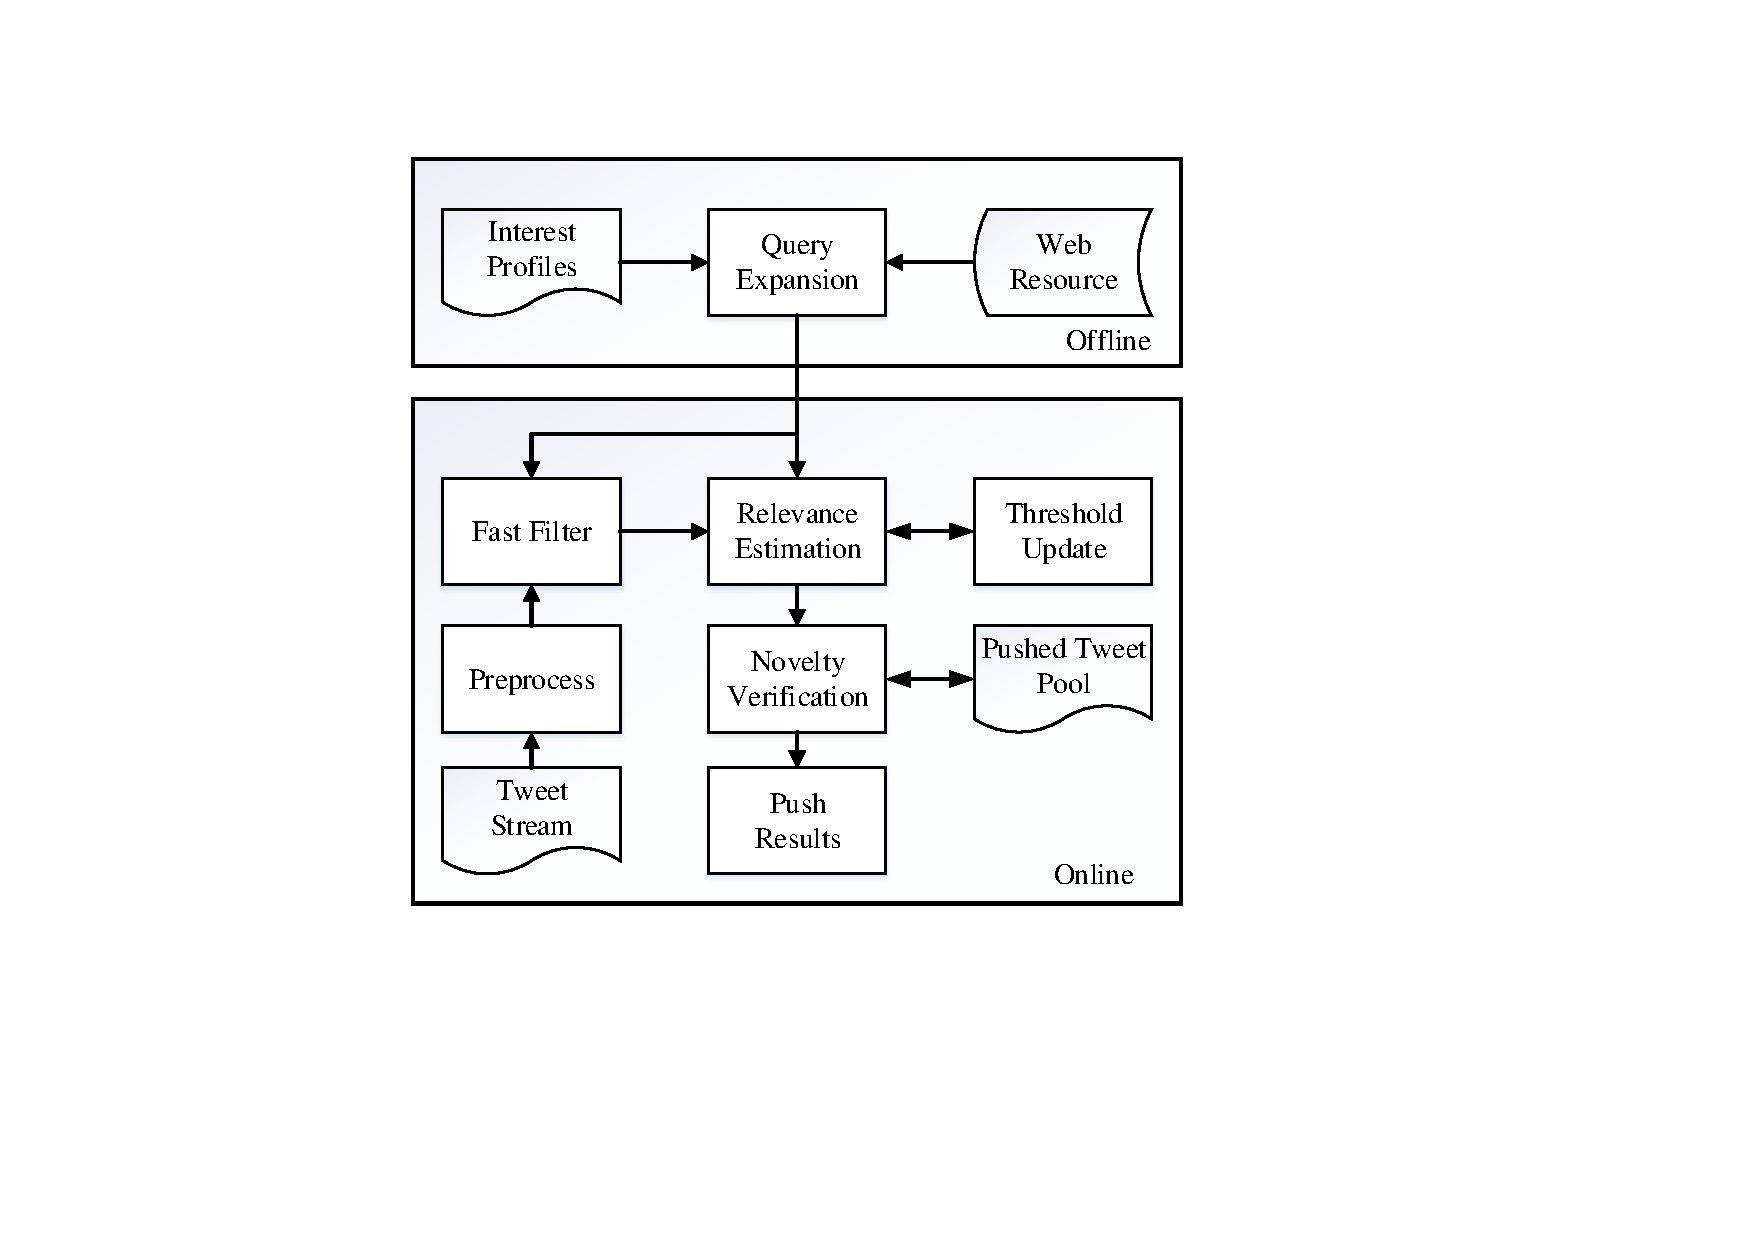
\epsfig{file=figures/scenarioA.pdf,width=0.45\textwidth}
}
\caption{Scenario A System Framework.}
\label{fig:Asys}
\end{figure}

\section{Scenario A: Push Notifications}
As previously mentioned, the goal of push notifications is to recommend relevant and
novel tweets based on the user’s interest profile in real-time.
At a high level, push notifications should be relevant (on topic),
timely (provide updates as soon after the actual event occurrence as possible),
and novel (users should not be pushed multiple notifications that say the same thing).
In this section, we mainly describe the architecture of our proposed system, which is shown in \ref{fig:a}.

\begin{figure}[htbp]
\centering {
	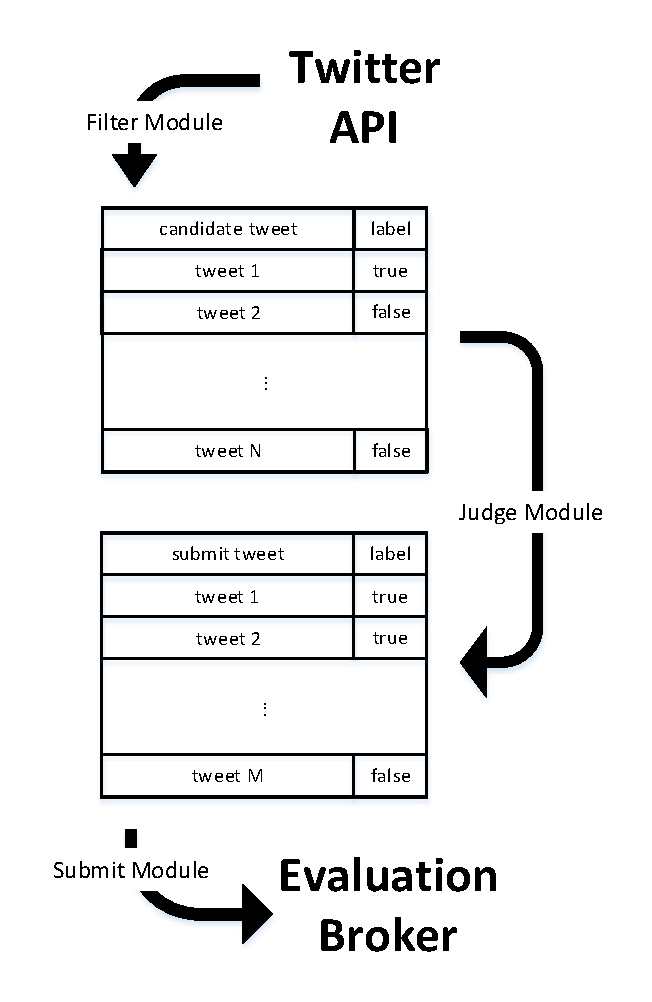
\epsfig{file=figures/a.pdf, width=0.35\textwidth}
}
\caption{The System Architecture of the Push Notifications Scenario.}
\label{fig:a}
\end{figure}

From the figure, we can observe that our system mainly contains three processes and two storage tables:

\begin{itemize}
\item \textbf{Filter Module:} 
In order to accelerate the speed of identifying possible relevant tweets for each profile,
We first build a interest vocabulary based on all words in the given users' interest profiles.
Then, the Twitter sample stream is obtained via the Twitter API.
For each crawled tweet, we check whether it contains any words in our interest vocabulary.
If contains, we insert it into our candidate tweets storage table. If not, filter it.
In this way, we simply ignore tweets that do not contain any keywords for each profile.

\item \textbf{Judge Module:}
This process keeps ``listening'' to the candidate tweets storage table.
In every $T1$, it selects at most $K1$ untreated candidate tweets and compare them with the given users' interest profiles.
For each (tweet, profile) pair, we first calculate the relevant score between them by the text similarity function $f$.
If the relevant scroe is bigger than $\alpha$, we then compute similarity scores between this tweet and all pushed tweets of this profile
via the text similarity function $f$, the biggest one will be chosen as the novel scroe.
If the novel score is smaller than $\beta$, we will insert it into the submission tweets storage table.
In the last, these selected tweets will be set to treated or removed from the storage table.

\item \textbf{Submit Module:}
This process keeps ``listening'' to the submission tweets storage table.
In every $T2$, it selects at most $K2$ untreated submission tweets and try to submit them to the evalation broker one by one.
If return code is $204$ for one tweet, which means the remote server accepted it successfully,
we will set the submitted tweet treated or remove it from the storage table.
Otherwise, the tweet is going to handle in the next round until accepted.
\end{itemize}

\subsection{Similarity Algorithm}
We utilize the KL-divergence language model for $f$ and $g$ to measure the relevance between
query language model $\widehat{\theta}_Q$ and tweet language model $\widehat{\theta}_D$
with the help of collection lanuage model $\widehat{\theta}_C$.
The smoothing methods we use for language model are:

(a) Jelinek-Mercer Smoothing
\begin{equation}
\begin{aligned}
JM(Q,&T,C) = \sum_{w \in Q} P(w|\widehat{\theta}_Q) \cdot \\
&log \left( (1-\lambda) * P(w|\widehat{\theta}_T) + \lambda * P(w|\widehat{\theta}_C) \right)
\end{aligned}
\end{equation}

(b) Dirichlet Smoothing
\begin{equation}
DIR(Q,T,C) = JM(Q,T,C), \lambda = \frac{\mu}{|T| + \mu}
\end{equation}

\subsection{Parameter Selection}
The $T1$ and $T2$ are both set to $10$ seconds.
$K1$ is set to $1000$ while $K2$ is set to $10$ due to their different scale.
Those parameters are set empirically and mainly depend on your computer performance.
$\alpha$ and $\beta$ are tuned via grid search on TREC 2015 dataset,
which is showed in Table \ref{tab:paraA}.

\begin{table}[htbp]
\centering
\caption{Parameters in the Email Digest Scenario.}
\label{tab:paraA}
\begin{tabular}{lccc}
\hline
Run ID&f&\alpha&\beta\\
\hline
PKUICSTRunA1&JM(\lambda=0.2)&0.79&0.72\\
PKUICSTRunA2&JM(\lambda=0.5)&0.85&0.74\\
PKUICSTRunA3&DIR(\mu=100)&0.75&0.68\\
\hline
\end{tabular}
\end{table}



\section{Scenario B: Email Digest}
In the email digest scenario,
we will identify a batch of up to 100 ranked tweets per day per interest profile.
At a high level, these results should be relevant and novel.
Timeliness is not important as long as the tweets were all posted on the previous day.

As shown in Fig.\ref{fig:Bsys}, our system for this scenario mainly contains four modules:

\begin{figure}[htbp]
\centering{
	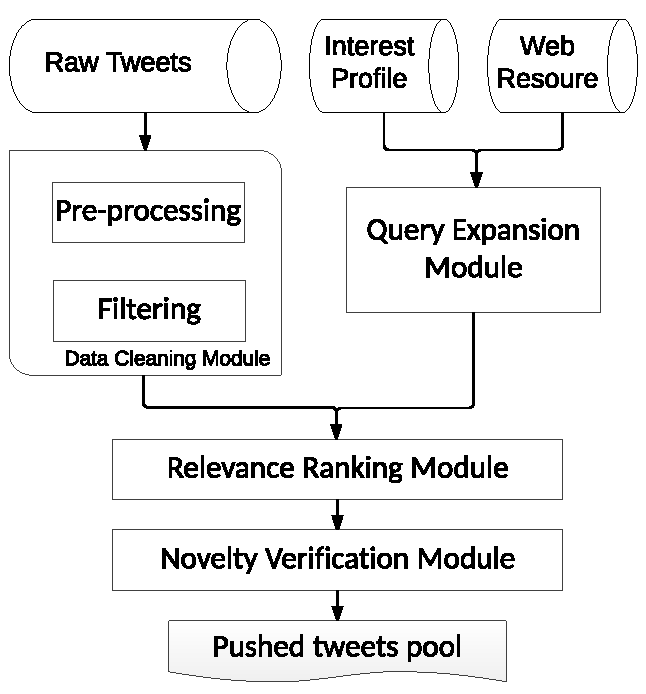
\epsfig{file=figures/b.pdf,width=0.4\textwidth}
}
\caption{The System Architecture of the Email Digest Scenario.}
\label{fig:Bsys}
\end{figure}

\begin{itemize}
\item \textbf{Data Cleaning Module:}
We preprocess all tweets during evaluation period.
And we simply filter tweets that do not contain any keywords for each interest profile,
and the rest tweets are chosen as candidate tweet collection,
which will accelerate identifying possible relevant tweets for each profile.

\item \textbf{Query Expansion Module:}
As microblog retrieval suffers severely from the vocabulary mismatch problem
(i.e. term overlap between query and tweet is relatively small).
To tackle this issue, we leverage web-based query expansion method to improve retrieval performance.
As is known to all, Google search is the dominant search engine in the majority countries
over the world, which indexes billions\cite{arlington2008google} of web pages,
so that users can search for the information they desire through the use of keywords and operators.
Therefore, we take the interest profile as the keywords to search in Google with Google Search Engine API before the evaluation period.
As the user interest profile offered by TREC 2016 are JSON-formatted structure and each profile includes four fields, topid, title, description and narrative.
Here we only use the topic keywords as our \emph{OriginQuery} since we utilize external web resource to depict the background information, noted as \emph{ExpansionQuery}.
We utilize the expanded query to represent the interest profile and then estimate the relevance between the query and tweets.

\item \textbf{Relevance Ranking Module:}
Similar with the push notifications scenario,
we utilize the text similarity function $f$ to measure the relevance between query and tweet.
Then, all the tweets are ranked based on their relevance score.

\item \textbf{Novelty Verfication Module:}
Once we obtain the ranked tweet list after relevance ranking,
we will traverse over them and judge novelty for each tweet,
until we collect enough tweets (the count of pushed tweets is up to $100$).
We use the text similarity function $g$ to measure the novelty between tweet
and the pushed tweets of interest profile.
When the novelty score is smaller than $\gamma$,
we think the tweet is a novel one for current interest profile and should be pushed.
In this module, there are two kinds of strategies to measure novelty between tweets:
(1) Negative KL-divergence. The higher relevance score between tweets, the less novelty they are.
(2) Simhash. It is a popular method to handle web page redundancy\cite{charikar2002similarity}.
Simhash is one where similiar items are hashed to similiar hash values
and we can calculate the bitwise hamming distance between hash values.
The closer hamming distance between two tweets is, the more similar they are.
The simhash code is calculated as follow,

\begin{equation}
\label{equ:lm}
Sim_{code} = sign(\sum_{i=1 \in n} w_{i} c_{i})
\end{equation}

where $w_{i}$ is the weight of term $i$ and $c_{i}$ is the hash code of term $i$, $sign$ is symbol function that make positive to 1 and negative to 0 for every bit in code.

\end{itemize}

\subsection{Parameter Selection}
$\gamma$ is tuned via grid search on TREC 2015 dataset,
which is showed in Table \ref{tab:paraB}.

\begin{table}[htbp]
\centering
\caption{Parameters of the Email Digest Scenario.}
\label{tab:paraB}
\begin{tabular}{lccc}
\hline
Run ID&f&g&$\gamma$\\
\hline
PKUICSTRunB1&JM($\lambda=0.2$)&DIR($\mu=100$)&0.73\\
PKUICSTRunB2&DIR($\mu=100$)&DIR($\mu=100$)&0.72\\
PKUICSTRunB3&DIR($\mu=100$)&SimHash&0.42\\
\hline
\end{tabular}
\end{table}



\section{Experiment}
The evaluation of TREC 2016 Real-time Summarization track takes place from
August 2, 2016 UTC to August 11, 2016 UTC.
And there are 203 interest profiles which participants will be responsible for tracking.
During the evaluation period, participants must maintain a running system
that continuously monitors the tweet sample stream.

For the push notifications scenario, the primary evaluation metrics
include Expected Gain (EG) and Normalized Cumulative Gain (nCG).
In the EG1 and nCG1 variants of the metrics, on a ``silent day'',
the system receives a score of one (i.e., perfect score) if it does not push any tweets,
or zero otherwise. In the EG0 and nCG0 variants of the metrics, for a silent day,
all systems receive a gain of zero no matter what they do.
Table \ref{tab:resA} shows the performance of our submitted three runs.
We could observe that in every run, EG1 and nCG1 are much larger than EG0 and nCG0,
which means our proposed system could recognise the ``silent day''
and make no push actions to avoid bothering users.
We use different text similarity algorithms in different runs
but their performance are similar, which could tell the robustness
of the negative KL-divergence with different smoothing strategies.

\begin{table}[htbp]
\centering
\caption{Performance of the Push Notifications Scenario.}
\label{tab:resA}
\begin{tabular}{lrrrr}
\hline
Run ID&EG1&EG0&nCG1&nCG0\\
\hline
PKUICSTRunA1&0.2342&0.0342&\textbf{0.2447}&0.0447\\
PKUICSTRunA2&\textbf{0.2347}&\textbf{0.0400}&0.2433&\textbf{0.0487}\\
PKUICSTRunA3&0.2329&0.0311&0.2343&0.0325\\
\hline
\end{tabular}
\end{table}

Table \ref{tab:resB} reports our results for the email digest scenario.
The primary evaluation metric is nDCG1.
As it turns out, PKUICSTRunB3 significantly outperforms both other runs,
indicating that the Simhash method for novelty verification module is successful in identifying novel tweets.
Both PKUICSTRunB1 and PKUICSTRunB2 adopt the negative KL-divergence,
with DIR(Bayesian Smoothing with Dirichlet Priors) smoothing and JM(Jelinek-Mercer method) respectively.
And the uniform novel thresholds are $\gamma=0.73$ and $\gamma=0.72$ training on the TREC 15 dataset.
From Table \ref{tab:resB}, we can see that nDCG1 and nDCG0 are the same in PKUICSTRunB1 and PKUICSTRunB2,
which means on each ``silent day'', our system still pushed some tweets that are regarded as unrelated ones.
Obviously, the thresholds do not fit well. Further investigation and experiments are needed to solve this issue.

\begin{table}[htbp]
\centering
\caption{Performance of the Email Digest Scenario.}
\label{tab:resB}
\begin{tabular}{lrrr}
\hline
Run ID&nDCG1&nDCG0\\
\hline
PKUICSTRunB1&0.1423&0.1423\\
PKUICSTRunB2&0.1569&\textbf{0.1569}\\
PKUICSTRunB3&\textbf{0.2348}&0.0151\\
\hline
\end{tabular}
\end{table}



\section{Acknowledgments}
The work reported in this paper is supported by the National Natural Science Foundation of China Grant 61370116.
%\section{Conclusion}
In this paper, we present our systems for TREC 2016 Real-Time Summarization Track.
In the push notification scenario,
we pay main attention on designing a online system
for handling the real-time Twitter sample stream
and make proper push actions for each interest profile.
In the email digest scenario,
We apply web-based query expansion using language model to rank candidate tweets and
then we leverage two kinds of strategies to measure novelty between tweets.
Experimental results show our effectiveness and efficiency of our system in both tasks.




\bibliographystyle{aaai}
\bibliography{yelp}
\end{document}
